\section{绪论}
\subsection{引言}
略
\subsection{基本术语}
\begin{enumerate}[label=(\roman*)]
    \item 样本/示例-sample/instance
    \item 训练集-training data
    \item 测试集-testing data
    \item 标记-label 
    \item 样例-example:拥有label的instance
    \item 泛化-generalization
\end{enumerate}
\subsection{假设空间}
\subsubsection{科学推理}
\begin{itemize}
    \item 归纳--induction
    从具体的事实归结出一般性规律
    \item 演绎--deduction
    从基础原理推演出具体状况
\end{itemize}
\subsubsection{归纳学习--inductive learning}
\begin{itemize}
    \item 广义归纳学习
    \item 狭义归纳学习--概念学习
    eg:布尔概念学习
\end{itemize}
\subsubsection{版本空间--version space}
即存在着一个与训练集一致的"假设集合"
\subsection{归纳偏好}
有多个与训练集一致的假设,但测试新样本时有不同的输出结果,那么采用哪种模型(假设)?
\subsubsection{"奥卡姆剃刀"原则}
若有多个假设与观察一致,则选最简单的那个.
利用什么原则,取决于算法能否获得更好的性能,泛化能力是否更强
\subsubsection{NFL(No Free Lunch Theorem)定理--"没有免费的午餐"定理}

\begin{theorem}[No Free Lunch 定理]\label{thm:nfl}
    对于所有学习算法 $\mathcal{L}_a$ 和 $\mathcal{L}_b$,在均匀分布的目标函数空间下,它们的训练外误差满足:
    \[
    \sum_f E_{ote}(\mathcal{L}_a|X,f) = \sum_f E_{ote}(\mathcal{L}_b|X,f)
    \]
\end{theorem}
\begin{proof}
    \begin{proofstep}[定义与假设]\label{step:def}
    假设样本空间 $\mathcal{X}$ 和假设空间 $\mathcal{H}$ 是离散的。定义:
    \[
    E_{ote}(\mathcal{L}_a|X,f) = \sum_{h \in \mathcal{H}} \sum_{x \in \mathcal{X} - X} P(x) \cdot \mathbb{I}(h(x) \neq f(x)) \cdot P(h|X,\mathcal{L}_a)
    \]
    其中 $\mathbb{I}(\cdot)$ 为指示函数。
    \end{proofstep}
    
    \begin{proofstep}[总误差求和]\label{step:sum}
    对所有目标函数求和:
    \begin{equation}
    \sum_f E_{ote}(\mathcal{L}_a|X,f) = \sum_f \sum_h \sum_{x \in \mathcal{X}- X} P(x)\mathbb{I}(h(x)\neq f(x))P(h|X,\mathcal{L}_a)
    \end{equation}
    \end{proofstep}
    
    \begin{proofstep}[交换求和顺序]\label{step:swap}
    将 $\sum_f$ 移至内部:
    \begin{align}
    &= \sum_{x \in \mathcal{X}- X} P(x) \sum_h P(h|X,\mathcal{L}_a) \nonumber \\
    &\quad \times \underbrace{\sum_f \mathbb{I}(h(x)\neq f(x))}_{\text{\highlight{\text{关键项}}}} \label{eq:keyterm}
    \end{align}
    \end{proofstep}
    
    \begin{proofstep}[计算关键项]\label{step:key}
    对于二分类问题,每个 $x$ 处的 $f(x)$ 有等概率取 0 或 1:
    \[
    \sum_f \mathbb{I}(h(x)\neq f(x)) = \frac{1}{2} \cdot 2^{|\mathcal{X}|} = 2^{|\mathcal{X}|-1}
    \]
    \end{proofstep}
    
    \begin{proofstep}[最终化简]\label{step:final}
    代入关键项并利用 $\sum_h P(h|X,\mathcal{L}_a) = 1$:
    \[
    \text{原式} = 2^{|\mathcal{X}|-1} \sum_{x \in \mathcal{X}- X} P(x)
    \]
    该结果与算法 $\mathcal{L}_a$ 无关,故对任意 $\mathcal{L}_a, \mathcal{L}_b$:
    \[
    \sum_f E_{ote}(\mathcal{L}_a|X,f) = \sum_f E_{ote}(\mathcal{L}_b|X,f)
    \]
    \end{proofstep}
\end{proof}
由\ref{thm:nfl}可知,脱离具体问题,空谈"什么学习算法最好"是毫无意义的
\subsection{发展历程}
推理期:1950s-1970s--符号知识,演绎推理

知识期:1970s中期--符号知识,领域知识

学习期:1980s--机器学习,归纳逻辑程序设计(Inductive Logic Programming)

统计学习:1990s中期--向量机(Support Vector Machine),核方法(Kernel Methods)

深度学习:2000s--神经网络

\subsection{应用现状}
信息科学,自然科学\dots

\subsection{阅读材料}
\subsubsection{机器学习}
国际会议:ICML,NIPS,COLT,ECML(Europe),ACML(Asia)

国际期刊:JMLR,ML

国内会议:CCML,MLA

\subsubsection{人工智能}
国际会议:IJCAI,AAAI

国际期刊:AI,JAIR

\subsubsection{数据挖掘}
国际会议:KDD,ICDM

国际期刊:ACM-TKDD,DMKD

\subsubsection{计算机视觉}
CVPR(会议),IEEE-TPAMI(期刊)

\subsubsection{神经网络}
期刊:NC,IEEE-TNNLS
\subsubsection{统计学}
期刊:AS

\subsection{习题}
\subsubsection{表1.1中若只包含编号为1和4的两个样例,试给出相应的版本空间.}
\begin{figure}[H]
    \centering
    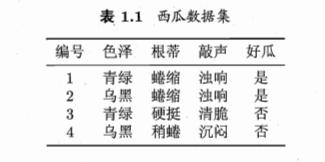
\includegraphics[width=0.8\textwidth]{static/images/西瓜数据集.png}
    \label{table:watermelon-data}
    \caption{表1.1西瓜数据集}
\end{figure}
解:
\begin{table}[ht]
    \centering
    \caption{\text{版本空间表}}
    \label{tab:logic-expressions}
    \begin{tabular}{cccc}
    \toprule
    \text{色泽} & \text{根蒂} & \text{敲声} & \text{逻辑表达式} \\
    \midrule
    \text{青绿} & \text{瓣缩} & \text{浊响} & $(\text{色泽} = \text{青绿}) \land (\text{根蒂} = \text{瓣缩}) \land (\text{敲声} = \text{浊响})$ \\
    \text{青绿} & \text{瓣缩} & * & $(\text{色泽} = \text{青绿}) \land (\text{根蒂} = \text{瓣缩})$ \\
    \text{青绿} & * & \text{浊响} & $(\text{色泽} = \text{青绿}) \land (\text{敲声} = \text{浊响})$ \\
    * & \text{瓣缩} & \text{浊响} & $(\text{根蒂} = \text{瓣缩}) \land (\text{敲声} = \text{浊响})$ \\
    \text{青绿} & * & * & $(\text{色泽} = \text{青绿})$ \\
    \bottomrule
    \end{tabular}
\end{table}
\subsubsection{估算共有多少种可能的假设}
与使用单个合取式来进行假设表示相比,使用“析合范式”将使得假设空间具有更强的表示能力。例如

好瓜 $\Leftrightarrow\left(\right.$ \textnormal{色泽} $=\star)\wedge($ \textnormal{根蒂} $=$ \textnormal{蜷缩} $\wedge$ \textnormal{敲声} $=\star)$

$\vee\left(\right.$ \textnormal{色泽} $=$ \textnormal{乌黑} $\wedge$\textnormal{ 根蒂} $=\star) \wedge$ \textnormal{敲声} $=$ \textnormal{沉闷} $\left.\right)$,

会把 “(色泽 = 青绿) ∧ (根蒂 = 蜷缩) ∧ (敲声 = 清脆)” 以及 “(色泽 = 乌黑) ∧ (根蒂 = 硬挺) ∧ (敲声 = 沉闷)” 都分类为 “好瓜”。
若使用最多包含 k 个合取式的析合范式来表达表 1.1 西瓜分类问题的假设空间,试估算共有多少种可能的假设。

解:色泽包含两种情况(青绿,乌黑),三种选择(青绿,乌黑,*);\\ 根蒂(蜷缩,稍蜷,硬挺)共4种选择;\\ 敲声(浊响/沉闷/清脆)共4种选择;
\par 除了不能存在(*,*,*)的组合,共包含$ 3 \times 4 \times 4 -1 = 47$种组合.\\ 题目求k个合取式的所有可能的组合之和,则有
\begin{equation}
    \boxed{\sum_{i}^{k} \binom{47}{i}}
\end{equation}
\subsubsection{若数据包含噪声,则假设空间中有可能不存在与所有训练样本都一致的假设。在此情形下,试设计一种归纳偏好用于假设选择。}
解:刚入门,可能无法正确回答此问题,但存在的方法应该有权重噪声注入/梯度稳定性惩罚/稀疏性偏好/集成鲁棒性.

\subsubsection{试证明“没有免费的午餐定理”仍成立。}
本章 1.4 节在论述“没有免费的午餐”定理时,默认使用了“分类错误率”作为性能度量来对分类器进行评估。若换用其他性能度量 \( \ell \),则式(1.1)将改为

\[ E_{ote}(\mathcal{L}_a | X, f) = \sum_h \sum_{x \in \mathcal{X} - X} P(x) \ell(h(x), f(x)) P(h | X, \mathcal{L}_a) \]

试证明“没有免费的午餐定理”仍成立。
\begin{proof}
    \begin{proofstep}
        性能度量虽发生了改变,目标函数仍然均匀分布,总误差表达式为:
        \begin{align*}
            E_{ote}(\mathcal{L}_a | X, f) &= \sum_h \sum_{x \in \mathcal{X} - X} P(x) \ell(h(x), f(x)) P(h | X, \mathcal{L}_a)\\
            &=\sum_{x \in \mathcal{X}-X}P(x) \sum_h P(h | X, \mathcal{L}_a) \sum_f \ell(h(x), f(x))
        \end{align*}
    \end{proofstep}
    \begin{proofstep}
       由\ref{thm:nfl}证明过程可知:$\sum_{f} f(x)=2^{|\mathcal{X}|-1}$
       \begin{equation}
        \therefore 
        \sum_f \ell(h(x), f(x)) = 2^{|\mathcal{X}|-1} \left[ \ell(h(x), 0) + \ell(h(x), 1) \right].
       \end{equation}
    \end{proofstep}
    \begin{proofstep}
        \begin{equation}
            \because P(h(x) = 0 | X, \mathcal{L}_a) = P(h(x) = 1 | X, \mathcal{L}_a) = \frac{1}{2}.
            \therefore  \sum_h P(h | X, \mathcal{L}_a) \left[ \ell(h(x), 0) + \ell(h(x), 1) \right] = \frac{1}{2} \left[ \ell(0, 0) + \ell(0, 1) + \ell(1, 0) + \ell(1, 1) \right].
        \end{equation}

        此结果与算法 \(\mathcal{L}_a\) 无关。
    \end{proofstep}
    \begin{equation}
        \sum_f E_{\text{ote}}(\mathcal{L}_a | X, f) = 2^{|\mathcal{X}|-1} \cdot \frac{1}{2} \sum_{x \in \mathcal{X} - X} P(x) \left[ \ell(0, 0) + \ell(0, 1) + \ell(1, 0) + \ell(1, 1) \right].
    \end{equation}
\end{proof}
无论选择何种性能度量 \(\ell\),只要真实目标函数 \( f \) 在所有可能的函数上均匀分布,无免费午餐定理仍然成立。算法的平均性能仅由数据分布和度量 \(\ell\) 的对称性决定,而与算法本身的设计无关。
\subsubsection{试述机器学习能在互联网搜索的哪些环节起什么作用。}
机器学习贯穿搜索的全流程,从理解用户意图到动态优化*\subsubsubsubsection{}结果,其核心价值在于通过数据驱动的方式提升搜索效率、准确性和个性化程度。知识库中提到的超参数优化(如随机搜索)、分布式表示(如协同过滤)等技术均为此提供了方法论支持。机器学习贯穿搜索的全流程,从理解用户意图到动态优化结果,其核心价值在于通过数据驱动的方式提升搜索效率、准确性和个性化程度。知识库中提到的超参数优化(如随机搜索)、分布式表示(如协同过滤)等技术均为此提供了方法论支持。
机器学习贯穿搜索的全流程,从理解用户意图到动态优化结果,其核心价值在于通过数据驱动的方式提升搜索效率、准确性和个性化程度。知识库中提到的超参数优化(如随机搜索)、分布式表示(如协同过滤)等技术均为此提供了方法论支持。